\documentclass[12pt,twoside]{article}
\usepackage[dvipsnames]{xcolor}
\usepackage{tikz,graphicx,amsmath,amsfonts,amscd,amssymb,bm,cite,epsfig,epsf,url}
\usepackage[hang,flushmargin]{footmisc}
\usepackage[colorlinks=true,urlcolor=blue,citecolor=blue]{hyperref}
\usepackage{amsthm,multirow,wasysym,appendix}
\usepackage{array,subcaption} 
% \usepackage[small,bf]{caption}
\usepackage{bbm}
\usepackage{pgfplots}
\usetikzlibrary{spy}
\usepgfplotslibrary{external}
\usepgfplotslibrary{fillbetween}
\usetikzlibrary{arrows,automata}
\usepackage{thmtools}
\usepackage{blkarray} 
\usepackage{textcomp}
\usepackage[left=0.8in,right=1.0in,top=1.0in,bottom=1.0in]{geometry}
\usepackage[left=0.8in,right=1.0in,top=1.0in,bottom=1.0in]{geometry}
\newcommand{\red}[1]{{\leavevmode\color{red}{#1}}}
\newcommand{\blue}[1]{{\leavevmode\color{blue}{#1}}}
\usepackage{graphicx}
%% Probability operators and functions
%
% \def \P{\mathrm{P}}
\def \P{\mathrm{P}}
\def \E{\mathrm{E}}
\def \Var{\mathrm{Var}}
\let\var\Var
\def \Cov {\mathrm{Cov}} \let\cov\Cov
\def \MSE {\mathrm{MSE}} \let\mse\MSE
\def \sgn {\mathrm{sgn}}
\def \R {\mathbb{R}}
\def \C {\mathbb{C}}
\def \N {\mathbb{N}}
\def \Z {\mathbb{Z}}
\def \cV {\mathcal{V}}
\def \cS {\mathcal{S}}

\newcommand{\RR}{\ensuremath{\mathbb{R}}}

\DeclareMathOperator*{\argmin}{arg\,min}
\DeclareMathOperator*{\argmax}{arg\,max}
\newcommand{\red}[1]{\textcolor{red}{#1}}
\newcommand{\blue}[1]{\textcolor{blue}{#1}}
\newcommand{\green}[1]{\textcolor{ForestGreen}{ #1}}
\newcommand{\fuchsia}[1]{\textcolor{RoyalPurple}{ #1}}

\newcommand{\wrnd}[1]{\widetilde{ #1 } }
\newcommand{\po}{\wrnd{\op{po}}  }

%
%% Probability distributions
%
%\def \Bern    {\mathrm{Bern}}
%\def \Binom   {\mathrm{Binom}}
%\def \Exp     {\mathrm{Exp}}
%\def \Geom    {\mathrm{Geom}}
% \def \Norm    {\mathcal{N}}
%\def \Poisson {\mathrm{Poisson}}
%\def \Unif    {\mathrm {U}}
%
\DeclareMathOperator{\Norm}{\mathcal{N}}

\newcommand{\bdb}[1]{\textcolor{red}{#1}}

\newcommand{\ml}[1]{\mathcal{ #1 } }
\newcommand{\wh}[1]{\widehat{ #1 } }
\newcommand{\wt}[1]{\widetilde{ #1 } }
\newcommand{\conj}[1]{\overline{ #1 } }
\newcommand{\rnd}[1]{\tilde{ #1 } }
\newcommand{\rv}[1]{ \rnd{ #1}  }
\newcommand{\rM}{\rnd{ m}  }
\newcommand{\rx}{\rnd{ x}  }
\newcommand{\ry}{\rnd{ y}  }
\newcommand{\rz}{\rnd{ z}  }
\newcommand{\ra}{\rnd{ a}  }
\newcommand{\rb}{\rnd{ b}  }
\newcommand{\rt}{\rnd{ t}  }
\newcommand{\rs}{\rnd{ s}  }


\newcommand{\rpc}{\widetilde{ pc}  }
\newcommand{\rndvec}[1]{\vec{\rnd{#1}}}

\def \cnd {\, | \,}
\def \Id { I }
\def \J {\mathbf{1}\mathbf{1}^T}

\newcommand{\op}[1]{\operatorname{#1}}
\newcommand{\setdef}[2]{ := \keys{ #1 \; | \; #2 } }
\newcommand{\set}[2]{ \keys{ #1 \; | \; #2 } }
\newcommand{\sign}[1]{\op{sign}\left( #1 \right) }
\newcommand{\trace}[1]{\op{tr}\left( #1 \right) }
\newcommand{\tr}[1]{\op{tr}\left( #1 \right) }
\newcommand{\inv}[1]{\left( #1 \right)^{-1} }
\newcommand{\abs}[1]{\left| #1 \right|}
\newcommand{\sabs}[1]{| #1 |}
\newcommand{\keys}[1]{\left\{ #1 \right\}}
\newcommand{\sqbr}[1]{\left[ #1 \right]}
\newcommand{\sbrac}[1]{ ( #1 ) }
\newcommand{\brac}[1]{\left( #1 \right) }
\newcommand{\bbrac}[1]{\big( #1 \big) }
\newcommand{\Bbrac}[1]{\Big( #1 \Big)}
\newcommand{\BBbrac}[1]{\BIG( #1 \Big)}
\newcommand{\MAT}[1]{\begin{bmatrix} #1 \end{bmatrix}}
\newcommand{\sMAT}[1]{\left(\begin{smallmatrix} #1 \end{smallmatrix}\right)}
\newcommand{\sMATn}[1]{\begin{smallmatrix} #1 \end{smallmatrix}}
\newcommand{\PROD}[2]{\left \langle #1, #2\right \rangle}
\newcommand{\PRODs}[2]{\langle #1, #2 \rangle}
\newcommand{\der}[2]{\frac{\text{d}#2}{\text{d}#1}}
\newcommand{\pder}[2]{\frac{\partial#2}{\partial#1}}
\newcommand{\derTwo}[2]{\frac{\text{d}^2#2}{\text{d}#1^2}}
\newcommand{\ceil}[1]{\lceil #1 \rceil}
\newcommand{\Imag}[1]{\op{Im}\brac{ #1 }}
\newcommand{\Real}[1]{\op{Re}\brac{ #1 }}
\newcommand{\norm}[1]{\left|\left| #1 \right|\right| }
\newcommand{\norms}[1]{ \| #1 \|  }
\newcommand{\normProd}[1]{\left|\left| #1 \right|\right| _{\PROD{\cdot}{\cdot}} }
\newcommand{\normTwo}[1]{\left|\left| #1 \right|\right| _{2} }
\newcommand{\normTwos}[1]{ \| #1  \| _{2} }
\newcommand{\normZero}[1]{\left|\left| #1 \right|\right| _{0} }
\newcommand{\normTV}[1]{\left|\left| #1 \right|\right|  _{ \op{TV}  } }% _{\op{c} \ell_1} }
\newcommand{\normOne}[1]{\left|\left| #1 \right|\right| _{1} }
\newcommand{\normOnes}[1]{\| #1 \| _{1} }
\newcommand{\normOneTwo}[1]{\left|\left| #1 \right|\right| _{1,2} }
\newcommand{\normF}[1]{\left|\left| #1 \right|\right| _{\op{F}} }
\newcommand{\normLTwo}[1]{\left|\left| #1 \right|\right| _{\ml{L}_2} }
\newcommand{\normNuc}[1]{\left|\left| #1 \right|\right| _{\ast} }
\newcommand{\normOp}[1]{\left|\left| #1 \right|\right|  }
\newcommand{\normInf}[1]{\left|\left| #1 \right|\right| _{\infty}  }
\newcommand{\proj}[1]{\mathcal{P}_{#1} \, }
\newcommand{\diff}[1]{ \, \text{d}#1 }
\newcommand{\vc}[1]{\boldsymbol{\vec{#1}}}
\newcommand{\rc}[1]{\boldsymbol{#1}}
\newcommand{\vx}{\vec{x}}
\newcommand{\vy}{\vec{y}}
\newcommand{\vz}{\vec{z}}
\newcommand{\vu}{\vec{u}}
\newcommand{\vv}{\vec{v}}
\newcommand{\vb}{\vec{\beta}}
\newcommand{\va}{\vec{\alpha}}
\newcommand{\vaa}{\vec{a}}
\newcommand{\vbb}{\vec{b}}
\newcommand{\vg}{\vec{g}}
\newcommand{\vw}{\vec{w}}
\newcommand{\vh}{\vec{h}}
\newcommand{\vbeta}{\vec{\beta}}
\newcommand{\valpha}{\vec{\alpha}}
\newcommand{\vgamma}{\vec{\gamma}}
\newcommand{\veta}{\vec{\eta}}
\newcommand{\vnu}{\vec{\nu}}
\newcommand{\rw}{\rnd{w}}
\newcommand{\rvnu}{\vc{\nu}}
\newcommand{\rvv}{\rndvec{v}}
\newcommand{\rvw}{\rndvec{w}}
\newcommand{\rvx}{\rndvec{x}}
\newcommand{\rvy}{\rndvec{y}}
\newcommand{\rvz}{\rndvec{z}}
\newcommand{\rvX}{\rndvec{X}}


\newtheorem{theorem}{Theorem}[section]
% \declaretheorem[style=plain,qed=$\square$]{theorem}
\newtheorem{corollary}[theorem]{Corollary}
\newtheorem{definition}[theorem]{Definition}
\newtheorem{lemma}[theorem]{Lemma}
\newtheorem{remark}[theorem]{Remark}
\newtheorem{algorithm}[theorem]{Algorithm}

% \theoremstyle{definition}
%\newtheorem{example}[proof]{Example}
\declaretheorem[style=definition,qed=$\triangle$,sibling=definition]{example}
\declaretheorem[style=definition,qed=$\bigcirc$,sibling=definition]{application}

%
%% Typographic tweaks and miscellaneous
%\newcommand{\sfrac}[2]{\mbox{\small$\displaystyle\frac{#1}{#2}$}}
%\newcommand{\suchthat}{\kern0.1em{:}\kern0.3em}
%\newcommand{\qqquad}{\kern3em}
%\newcommand{\cond}{\,|\,}
%\def\Matlab{\textsc{Matlab}}
%\newcommand{\displayskip}[1]{\abovedisplayskip #1\belowdisplayskip #1}
%\newcommand{\term}[1]{\emph{#1}}
%\renewcommand{\implies}{\;\Rightarrow\;}



\newcommand{\ru}{\rnd{ u}  }
\newcommand{\rd}{\rnd{ d}  }
%\newcommand{\rs}{\rnd{ s}  }
\newcommand{\ri}{\rnd{ i}  }
\newcommand{\re}{\rnd{ e}  }
\newcommand{\rQ}{\rnd{ q}  }
\newcommand{\rC}{\rnd{ c}  }


\begin{document}

\begin{center}
{\large{\textbf{Homework 4}} } \vspace{0.2cm}\\
Due October 10 at 11 pm
\\
\end{center}
Unless stated otherwise, justify any answers you give.
You can work in groups, but each
student must write their own solution based on their own
understanding of the problem.

When uploading your homework to Gradescope you will have to
select the relevant pages for each question.  Please submit each
problem on a separate page (i.e., 1a and~1b can be on the same page but 1
and 2 must be on different pages).  We understand that this may be
cumbersome but this is the best way for the grading team to grade your
homework assignments and provide feedback in a timely manner.  Failure
to adhere to these guidelines may result in a loss of points.
Note that it may take some time to
select the pages for your submission.  Please plan accordingly.  We
suggest uploading your assignment at least 30 minutes before the deadline
so you will have ample time to select the correct pages for your
submission.  If you are using \LaTeX, consider using the minted or
listings packages for typesetting code.  
\\

\begin{enumerate}

\item (Half life)
The half life of a radioactive substance is a way to quantify how rapidly the substance decays. Given a fixed quantity of the substance, the half time is the time that it takes for it to be reduced to half (i.e. half of the radioactive particles have decayed). It is not immediately apparent why the time should be the same for any quantity. Here we show that it is (probabilistically), as long the particles decay following an exponential distribution.  
\begin{enumerate}
\item Let $\rnd{t}$ be a random variable with a pdf of the form
\begin{align}
f_{\rnd{t}}(t) := \begin{cases}
\lambda \exp(- \lambda t), \qquad \text{if $t\geq 0$},\\
0 \qquad \text{otherwise},
\end{cases}
\end{align}
where $\lambda$ is a fixed constant. We define the half life $t_{1/2}$ as the number that satisfies $\P(\rnd{t} > t_{1/2}) = 1/2$. Compute $t_{1/2}$ in terms of $\lambda$. Then explain intuitively why this is a reasonable definition for the half life.
\blue{
\begin{itemize}
    \item we know that given a pdf $f_{\Tilde{t}}(t)$ the cdf will be defined as $F_{\Tilde{t}}(t)=\int_{-\infty}^{t}f_{\Tilde{t}}(t)dt=P(\Tilde{t}<t)$
    \item using this we can solve $F_{\Tilde{t}}(t)=\int_{-\infty}^{t}f_{\Tilde{t}}(a)da=\int_{0}^{t}f_{\Tilde{t}}(a)da=\int_{0}^{t}\lamda e^{-\lambda a}da=1-e^{-\lambda t}$
    \item then it is clear that $P(\Tilde{t}>t)=1-P(\Tilde{t}<t)=1-F_{\Tilde{t}}(t)$
    \item so we can find $\frac{1}{2}=1-F_{\Tilde{t}}(t)$ given us $\frac{1}{2}=1-1+e^{-\lambda t}$ meaning that $\frac{1}{2}=e^{-\lambda t}$ \item taking the log of both sides we get $-log(2)=-\lambda t$
    \item which finally yields $\frac{log(2)}{\lambda}=t_{\frac{1}{2}}$ 
    \item if we think of $\Tilde{t}$ as the mass of the substance. \item we know that the pdf is the rate of decay of the substance and $F_\Tilde{t}(t)$ is the amount of the substance that has decayed so far. 
    \item so once $F_\Tilde{t}(t)=\frac{1}{2}$ it means that half of the subtance has decayed
\end{itemize}

}
\item Compute $t$ such that $\P( t_{1/2} < \rnd{t} < t) = 1/4$, and express it in terms of only $t_{1/2}$. Explain why the result is consistent with the intuitive meaning of half life.
\blue{
\begin{itemize}
    \item we can see that $P(t_{\frac{1}{2}}<\Tilde{t}<t)=F_{\Tilde{t}}(t)-F_{\Tilde{t}}(t_{\frac{1}{2}})$ furhter by defention of half life we know that $F_{\Tilde{t}}(t)-F_{\Tilde{t}}(t_{\frac{1}{2}})=F_{\Tilde{t}}(t)-\frac{1}{2}$ and as we know the cdf we can express this as $F_{\Tilde{t}}(t)-\frac{1}{2}=1-e^{-\lambda t}-\frac{1}{2}=\frac{1}{2}-e^{-\lambda t}$ 
    \item finally we want to sovle $\frac{1}{4}=\frac{1}{2}-e^{-\lambda t}$ whcih simplfies to $\frac{1}{4}=e^{-\lambda t}$ 
    \item we can sovle this by taking logs on both sides and finally get $-\frac{log(4)}{\lambda}=t=2\frac{log(2)}{\lambda}$
    \item this can be thought of as we are looking for a t such that, the one foruth of the mass decays after the half life and before this t. 
    \item so this t can be thought of as the half life of the half life in effect, it is the time after the half life that it takes for half of the remaining substance to disintegrate. \item alternatively it could be thought of as the time it takes for $\frac{3}{4}$ of the substance to disintegrate.
    \item in other words it is 2 times the half life
\end{itemize}

}

\item Compute $\P( \rnd{t} > k t_{1/2} )$ for any integer $k$. Again, explain why the result is consistent with the intuitive meaning of half life.
\blue{
\begin{itemize}
    
\item as we know the pdf of $\tilde{t}$ we know that $F_{\Tilde{t}}(kt_{\frac{1}{2}})=1-e^{-\lambda kt_{\frac{1}{2}}}=1-e^{-\lambda k \frac{log(2)}{\lambda}}=1-e^{-log(2) k}$
\item further we know that $F_{\Tilde{t}}(t)=1-P(\tilde{t}<t)$
\item meaning  that we can find $P(t<\Tilde{kt_{\frac{1}{2}}})=1-F_{\Tilde{t}}(kt_{\frac{1}{2}})=1-(1-e^{-log(2) k})=e^{-log(2) k}=e^{-log(2^k)}=\frac{1}{2^k}$
\item this means that it takes another $T_{1/2}$ for half of the remaning mass to decay so it half its self at a constent rate 

\end{itemize}
}

\end{enumerate}

\item (Triangular pdf)
We are interested in fitting a model with a parametric pdf equal to
\begin{align}
f_{w}\brac{x}  = \begin{cases}
 \frac{2x}{w^2}, \qquad & \text{for } 0 \leq x \leq w,\\
0, \qquad & \text{otherwise},
\end{cases}
\end{align}
where the parameter $w$ is nonnegative. 
%\begin{comment}
%Both the pdf and the cdf are plotted in Figure~\ref{fig:triangle}.  
%\begin{figure}[tp]
%% Preamble: \pgfplotsset{width=7cm,compat=1.12}
%% \begin{center}
%\begin{tikzpicture}[scale=0.95]
%\begin{axis}[xmin= -0.1, xmax=2.1, ymin=-0.1, ymax=1.1,xlabel=$x$,
%ylabel=$f_{X} \brac{x }  $, xticklabels={0,w}, xtick={0,2},
%yticklabels={0,$\frac{2}{w}$}, ytick={0,1}]
%\addplot[blue, very thick, domain=0:2, samples=51] { x/2)};
%\addplot[blue, very thick, domain=-0.1:0, samples=2] {0};
%\addplot[blue, very thick, domain=2:2.1, samples=2] {0};
%\addplot[dashed, very thick, samples=2] coordinates {(2,0)(2,1)};
%\end{axis}
%\end{tikzpicture}
%%\end{center}
%\caption{Triangular pdf and the corresponding cdf.}
%\label{fig:triangle}
%\end{figure}
%\end{comment}

\begin{enumerate}
\item The observed values are 1.25, 0.4, 1.5, 1, 1.2. What are the possible values of the parameter $w$? 
\blue{
\begin{itemize}
    
\item w is non negative so it can range from 0 to infinity. 
\end{itemize}
}
\item Compute the likelihood function corresponding to these data and sketch it. 
\blue{
\begin{itemize}
    \item we know that the likelihood function is defined as  $ \mathcal{L}_{X}(w)=\Pi_{i=1}^{n}f_{\Tilde{w}}(x_i)=\Pi_{{i=1}}^{n}\frac{2x_i}{w^2}$
    \item  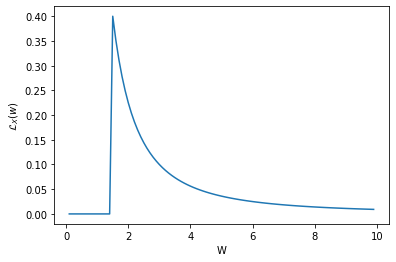
\includegraphics[width=15cm]{homework 4/question 2.png}
\end{itemize}

}
\item What is the maximum likelihood estimate of $w$? 
\blue{
\begin{itemize}
    \item we know that $\mathcal{L}_{X}(w)$ is a product so any value of w that produces $f_{w}(x_i)=0$ for any data point will have a likelihood of zero. thus any point with $w< max(x_1...x_n)$ will have a likelihood of zero. 
    \item if we instead consider just $w\geq max(x_1...x_n)$ we can take the log likelihood as  $log(\mathcal{L}_{X}(w))=\Sigma_{i=1}^{n}log(2x_i)-2log(w)$ 
    \item differentiating the log likelihood with respect to w we get $-\frac{2}{w}$ which is always negative. meaning that the likelihood is always decreasing 
    \item thus we know that $w_{ml}=max(x_1...x_n)$
\end{itemize}
}
\item  Assume that the data are indeed generated by the parametric model with $w:=w_{\op{true}}$. Does the ML estimate systematically underestimate or overestimate the true parameter? 
\blue{
\begin{itemize}
    

\item this will underestimate our data as we are sampling from a distribution and setting our parameter equal to the max value observed in that sample, but it is unlikely in any sample we will ever observe the true largest possible value of a random varibale, thus we systematical underestimate. 

\end{itemize}
}
\item Generate a sample from a random variable with this parametric distribution, where $w:=2$, using a uniform sample from the interval $\sqbr{0,1}$ equal to 0.64.
\blue{
\begin{itemize}
    \item we first want to find the cdf so $F_{\tilde{w}}(x)=\int_{-\infty}^{x}f_{\tilde{w}}(w)dw=\int_{0}^{x}f_{\tilde{w}}(w)dw=\int_{0}^{x}\frac{2w}{4}dw=\frac{w^2}{4}$ 
    \item more fomrally our cdf is $F_{\tilde{w}}(x)\left\{
    \begin{array}{lr}
        0 & \text{if} x< 0\\
        \frac{w^2}{4}, & \text{if} x\in[0,2]\\
        1 & \text{else}
    \end{array}$
    \item for a uniform rv, we are only dealing with values between 0 and 1. so we can just focous on teh middle case in this sitatuion $F_{\tilde{w}}^{-1}(\tilde{u})=2\sqrt{\Tilde{u}}$
    \item so we can see that$ x=F_{\tilde{w}}^{-1}(\tilde{u})=2\sqrt{.64}=2(.8)=1.6$
\end{itemize}
}
\end{enumerate}

\item (Planet)
An astrophysicist determines that a good model for the pdf of the temperature in a newly discovered planet is
\begin{align}
f_{\rnd{t}}(t) := \frac{\lambda \exp (-\lambda \abs{t})}{2},
\end{align}
where $t$ can be any real number (in particular it can be negative or positive).
\begin{enumerate}
\item Compute the cdf of $\rnd{t}$.
\blue{
\begin{itemize}
    \item first note that the $|x|$ is defined as $|x|=\left\{
    \begin{array}{lr}
        -x & \text{if} x< 0\\
        x & \text{otherwise}
    \end{array}$
    \begin{enumerate}
        \item so we have two cases 
        \item first if $t\leq 0$
        \begin{itemize}
            \item in this case $F_{\Tilde{t}}(t)=\int_{-\infty}^{t}f_{\Tilde{t}}(x)dx=\int_{-\infty}^{t}\frac{\lambda e^\lambda x}{2}$ = $\frac{1}{2}e^{\lambda x}|_{-\infty}^{t}=\frac{e^{\lambda t}}{2}$
        \end{itemize}
        \item on the other hand if $t\geq 0$ 
        \begin{itemize}
            \item in this case we have $F_{\Tilde{t}}(t)=\int_{-\infty}^{0}f_{\Tilde{t}}(x)dx+\int_{0}^{t}f_{\Tilde{t}}(x)dx=\int_{-\infty}^{0}\frac{\lambda e^\lambda x}{2}+\int_{0}^{t}\frac{\lambda e^-\lambda x}{2}$ = $1-\frac{e^{-\lambda t}}{2}$
        \end{itemize}
        \item so our ovall cdf is $F_{\Tilde{t}}(t)=\left\{
    \begin{array}{lr}
        \frac{e^{\lambda t}}{2} & \text{if} t< 0\\
        1-\frac{e^{-\lambda t}}{2} & \text{otherwise}
    \end{array}$
    \end{enumerate}
\end{itemize}}
\item Compute the maximum-likelihood estimate of $\lambda$ from the following data: 5, -50, -1, 100
\blue{
\begin{itemize}
    \item we know the loglickyhood function will be $\mathcal{L}_{X}(\lambda)=nlog(\lambda)-nlog(2)+\lambda\Sigma_{i=1}^{n}|x_i|$
    \item we can take the second darivative with respect to $\lambda$ and get $-\frac{n}{\lambda ^2}$ which is always less then zero, so any point where our first darivative is zero will be a global max 
    \item setting our first darivative with respect to $\lambda$ equal to zero we get $\frac{n}{\lambda}-\Sigma_{i=1}^{n}|x_i|=0$ meaning that $\frac{n}{\lambda}=\Sigma_{i=1}^{n}|x_i|$ and finally $\lambda_{ml}=\frac{n}{\Sigma_{i=1}^{n}|t_i|}$
    \item applying this to the data we get $\lambda_{ml,x}=\frac{4}{50+5+1+100}=\frac{4}{156}$
\end{itemize}

}
\item What is the pdf of $\rnd{t}$ conditioned on the event $\rnd{t}>0$?
\blue{
\begin{itemize}
    \item first we want to solve for the cdf of this case. 
    \item we can see that $P(\tilde{t}\leq t|\tilde{t}>0)=\frac{P(\tilde{t}\leq t\cap\tilde{t}>0)}{P(\tilde{t}>0)}=\frac{F_\tilde{t}(t)-F_\tilde{t}(0)}{1-F_\tilde{t}(0)}$ 
    \item we showed abovue that  $F_{\Tilde{t}}(t)=\left\{
    \begin{array}{lr}
        \frac{e^{\lambda t}}{2} & \text{if} t< 0\\
        1-\frac{e^{-\lambda t}}{2} & \text{otherwise}
    \end{array}$
    \item thus we have $P(\tilde{t}\leq t|\tilde{t}>0)=\frac{F_\tilde{t}(t)-F_\tilde{t}(0)}{1-F_\tilde{t}(0)}}$=$\frac{1-\frac{e^{\lambda t}}{2}-\frac{1}{2}}{1-\frac{1}{2}}=1-e^{-\lambda t}$
    \item then we can find the pdf as that quantity by difertniating $1-e^{-\lambda t}$ with respect to t, which yields $\lamda e^{-\lambda t}$ as our final solution.
    \item note that this means that $\tilde{t}$ is exponentially distributed when condtioned on being greater than zero.
\end{itemize}
}
\end{enumerate}

\item(Tempature)
The tables in \textit{train.csv} and \textit{test.csv} record the daily maximum temperature (TMAX) of Seattle.
\begin{enumerate}
    \item Estimate the pdf of TMAX with the following models on the training set. Compare the pdf with a normalized histogram in the test set. Which model performs better visually?
        \begin{itemize} 
            \item Estimating the parameter of Gaussian distribution with MLE;
            \item Non-parametric KDE with the Gaussian kernel at different bandwidths (e.g. 1, 2, 5).
        \end{itemize}
        \blue{
        \begin{itemize}
            \item  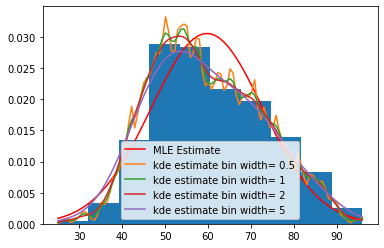
\includegraphics[width=15cm]{homework 4/question 4a.png}
            \item it seems that the kde estimate with bin width of 2 does the best
        \end{itemize}
        
        }
        
    \item Repeat the experiment only on \text{July} and \text{August} data. Which model performs better visually? Compare the results with (a) and explain your findings. 
    \blue{
        \begin{itemize}
            \item  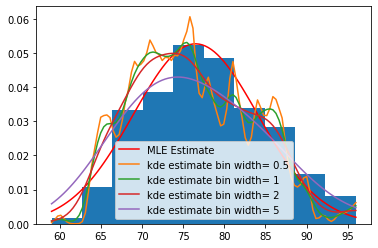
\includegraphics[width=15cm]{homework 4/question 4b.png}
            \item it seems that the mle esitmate does better 
            \item this makes sense as we are just rersticting our data to summer months and the data is more normally distributed during that time frame so a Guasian MLE fits the data well. 
        \end{itemize}
        
        }
\end{enumerate}

\end{enumerate}
\end{document}
